\documentclass{report}
\usepackage{setspace} % Setting line spacing
\usepackage{ulem} % Underline
\usepackage{caption} % Captioning figures
\usepackage{subcaption} % Subfigures
\usepackage{geometry} % Page layout
\usepackage{multicol} % Columned pages
\usepackage{array,etoolbox}
\usepackage{fancyhdr}
\usepackage{enumitem}
\usepackage[toc,page]{appendix}

% Page layout (margins, size, line spacing)
\geometry{letterpaper, left=1in, right=1in, bottom=1in, top=1in}
\setstretch{1.5}

% Headers
\pagestyle{fancy}
\lhead{PeaPod - Requirements}
\rhead{UpRoute Development Foundation}

% Metric counter, referencing commands
\newcounter{metricnumber}
\setcounter{metricnumber}{1}
\newcommand{\metricrow}{M\arabic{metricnumber}}
\newcommand{\mlabel}[1]{\addtocounter{metricnumber}{-1}\refstepcounter{metricnumber}\label{#1}\addtocounter{metricnumber}{1}}
\newcommand{\mref}[1]{M\ref{#1}}

\begin{document}

\begin{titlepage}
    \begin{center}
        \vspace*{1.2cm}

        \textbf{\large{PeaPod - Requirements}}

        \vspace{0.5cm}

        Outlining the Requirements for a Design Submission to the \\NASA/CSA Deep Space Food Challenge

        \vfill \small{

            \textbf{Jayden Lefebvre - Lead Engineer, Founder of UpRoute Development Foundation}\\
            BASc Computer Engineering (Anticipated 2024), University of Toronto\\
            Toronto, ON, Canada\\
            \vspace{.5cm}
            \textbf{Nathan Chareunsouk - Design Lead}\\Toronto, ON, Canada\\
            \vspace{.5cm}
            \textbf{Navin Vanderwert - Design Engineer}\\
            BASc Engineering Science (Anticipated 2024), University of Toronto\\
            Toronto, ON, Canada\\
            \vspace{.5cm}
            \textbf{Jonas Marshall - Electronics Engineer}\\
            BASc Computer Engineering (Anticipated 2024), Queen's University\\
            Kingston, ON, Canada

        }

        \vspace{1cm}

        Primary Contact Email: jayden.lefebvre@mail.utoronto.ca

        \vspace{.75cm}

        Revision 0.7\\
        UpRoute Development Foundation\\
        May 21st, 2021

    \end{center}
\end{titlepage}

\thispagestyle{plain}

\tableofcontents
\newpage

\section{Introduction}
\label{sec:intro}

\subsection{Purpose}
\label{sec:purpose}

The purpose of this document is to outline both the category requirements (Section \ref{sec:requirements}) for a design submission to the NASA/CSA Deep Space Food Challenge Phase 1 \cite{dsfc} and the scoped requirements (Section \ref{sec:scope}) for the design being proposed by University of Toronto Agritech (UTAG).

The goal of the Deep Space Food Challenge is for participants to "Create novel food production technologies or systems that require \uline{minimal inputs} and \uline{maximize safe, nutritious, and palatable food outputs} for \uline{long-duration space missions}, and which have potential to benefit people on Earth." \cite{applicantguide}

\subsection{Framing Structure}
\label{sec:structure}

This document achieves its purpose via "top-down" framing (Section \ref{sec:framing}), with each subsection's entries being derived from the entries of the
previous\footnote{Each objective and metric has a numbered reference to the entry it was derived from (\uline{\textbf{S}}takeholder \uline{\textbf{1}} : S1, \uline{\textbf{H}}igh-\uline{\textbf{L}}evel Objective \uline{\textbf{8}} : HL8, etc.)}.
\begin{itemize}
    \item \textbf{\ref{sec:opportunity} - Opportunity}: A succinct scoped challenge statement.
    \item \textbf{\ref{sec:requirements} - Challenge Requirements}: Categorical/unscoped requirements for \textit{any} submission.
    \item \textbf{\ref{sec:stakeholders} - Stakeholders}: Persons and groups in consideration.
    \item \textbf{\ref{sec:hlos} - High-Level Objectives}: Conceptual aims, DfX; derived from Requirements and Stakeholders.
    \item \textbf{\ref{sec:llos} - Low-Level Objectives}: Tactical goals; derived from HLOs.
    \item \textbf{\ref{sec:metrics} - Metrics}: Quantitative measures of design success, fit, utility, etc.; derived from LLOs.
    \item \textbf{\ref{sec:constraints} - Constraints}: Scoped \textit{mandatory} requirements for the proposed design.
    \item \textbf{\ref{sec:criteria} - Criteria}: Scoped \textit{graded} requirements for the proposed design.
\end{itemize}

% In addition to framing both the challenge space and our solution space, this document serves to outline the function and feature requirements of the Phase 1 prototypes (See Appendices \ref{sec:assessment}, \ref{sec:application}).

\newpage

\subsection{Scope and Justification}
\label{sec:scope}

The three underlined criteria in the challenge statement in Section \ref{sec:purpose} have also helped to define the scope of this document:
\begin{enumerate}[label=SC\arabic*., ref=SC\arabic*]
\item \label{sc:1} The longer the duration of the space mission (up to and including interplanetary travel and permanent colonization) the lesser the feasability of
    resupply\footnote{Minimal resupply is also listed as a constraint directly in the challenge details \cite{applicantguide}.}.
    The lesser the feasability of resupply, and the more minimal the input (i.e. launch mass), the less food will be able to be packed at launch, thus the more the design will need to generate \uline{net-new food grown on-board during the mission}.
\item \label{sc:2} The minimization of inputs (launch mass), the minimization of other negative criteria such as growth time, design complexity, etc. and the maximization of safety (pathogenic and otherwise) means that food animal growth has been deemed not feasible, and is outside the scope of this document. Thus, the design should focus on \uline{food-producing plant (or crop)
    growth}\footnote{This is primarily an issue in-transit; for colonization, non-plant food production systems should definitely be considered.}.
\item \label{sc:3} Spacecraft are not good crop growth systems (lack of water access, proper lighting and nutrition, etc.), thus the design should encompass a \uline{crop growth environment} that:
    \begin{enumerate}[label=SC3\alph*., ref=SC3\alph*]
        \item \label{sc:3a} provides of all necessary \uline{crop growth inputs} (water, nutrients, lighting, etc.);
        \item \label{sc:3b} contains or otherwise encompasses a viable \uline{crop growth environment} (temperature, humidity, gas concentrations, airflow, etc.);
        \item \label{sc:3c} has control over all \uline{parameters} of both a) and b) (environment parameters); these together are the (crop growth) \uline{environment conditions}.
    \end{enumerate}
\item \label{sc:4} To maximise safety (of both the crops and the crew) and redundancy, and to minimize inputs (required human interaction), the environment should be \uline{automated and isolated} from the spacecraft cabin with regards to all environment conditions (thermally, water-tight, etc.) unless beneficial and efficient (i.e no loss).
\newpage
\item \label{sc:5} A greater degree of nutrition and palatability of food outputs implies a greater variety of crops (incl. leafy greens, fruits/fruiting vegetables, root vegetables, algaes, etc.); as such the food production system should be able to \uline{generate a continuous and wide variety of environmental conditions} such that \uline{virtually any food crops} could be grown within.
\item \label{sc:6} The demand for high crop variety, automation, parameter control, efficiency/input minimization (water, nutrients, footprint per crop), etc. implies the use of an \uline{aeroponic crop growth method} \cite{spinoff}.
\item \label{sc:7} Output nutrient and yield maximization in a controlled-environment implies \uline{environment parameter optimization}. 
    This is best accomplished via data collection of both plant-growth and environment metrics and cross-growth-environment networking (data versatility, sharing, and machine intelligence).
\item \label{sc:8} A solution focussed on palatability (focus on enjoyable crops) and variety (adaptability to many distinct environment requirements) is not suited to high caloric output. 
    Most crops are simply not able of producing the required daily caloric output in the space alotted (Section \ref{sec:constraints}). 
    As such, the scope of our solution places \uline{far greater importance on output palatability and variety} (both culinary and nutritional) as well as production of critical micronutrients as opposed to pure caloric 
    yield\footnote{The solution "need not meet the full nutritional requirements of future crews, but can contribute significantly to, and integrate with, a comprehensive food system." \cite{applicantguide}}.
\end{enumerate}
Phase 1 development, testing, and assessment is scoped to terrestrial/Earth-like operational constraints \cite{applicantguide}:
\begin{itemize}
    \item Gravity (9.81 m/s${}^2$);
    \item Ambient atmospheric pressure (101,325 Pa);
    \item Ambient atmospheric temperature (22 °C);
    \item Ambient atmospheric humidity (50 \%RH);
\end{itemize}

\newpage
\subsection{Definitions}
\label{sec:definitions}

A number of useful definitions have emerged from the above scoping:
\begin{enumerate}
\item \textbf{(Crop Growth) Environment} - The environment within which the crop grows/with which the crop interacts; the Environment Parameters in terms of their relationship with the crop and its growth.
\item \textbf{(Crop Growth) Environment Parameters} - The (often quantitative) parameters of the Crop Growth Environment, as well as any and all other parameters influencing crop growth.
\item \textbf{Crop Growth System} - Includes the physical enclosure (containing the crops and the controlled environment; incl. isolation) as well as any infrastructure required to generate the crop growth environment and control all environment conditions; satisfies all requirements in this document.
\item \textbf{Crop Growth Metrics} - The (often quantitative) measures of crop growth optimization, including yield mass, growth rate, nutrient/etc. concentrations, etc.
\item \textbf{Environment Program} - The to-date most optimized set of Environment Parameters for a given Crop Growth Metric, implemented by the Grop Growth System.
\end{enumerate}

\newpage
\section{Framing}
\label{sec:framing}

\subsection{Opportunity}
\label{sec:opportunity}

Design an automated and isolated aeroponic crop growth system for the Deep Space Food Challenge Phase 1\cite{dsfc}, able to generate any environment from a combination of independent environment parameters, with both environment and crop growth data collection.

\subsection{Challenge Requirements}
\label{sec:requirements}

The following are the overall challenge requirements compiled from DSFC Applicant Guide details \cite{applicantguide} and an excerpt of NASA-STD-3001: Section 7.1 Food and Nutrition\footnote{Additional nutrition and caloric output constraints relative to activity level, crew details, etc. are provided; however they are not in direct consideration as of Phase 1.} \cite{nutrition}:
\begin{enumerate}[label=R\arabic*., ref=R\arabic*]
    \item \label{r:1} \textbf{Must} help fill food gaps for a \textit{three-year} round-trip mission with \textit{no resupply}:
    \begin{enumerate}[ref=R1\alph*]
        \item \label{r:1a} \textbf{Should} aim to produce food outputs that fulfill \textbf{all daily nutritional needs} for a crew of \textit{four (4)} people;
        \item \label{r:1b} \textbf{Must} maintain food output \textit{safety} and \textit{nutrition} during \textit{all phases} of the mission;
        \item \label{r:1c} \textbf{Must} output food that is \textit{varied, palatable, and acceptable} to the crew for the \textit{duration} of the mission;
        \item \label{r:1d} \textbf{Must} produce food outputs that require \textit{no additional processing 
        time}\footnote{It is assumed that fresh (or packaged unprepared) edible plant products are already prepared on existing space missions, and that this preparation meets this requirement.};
    \end{enumerate}
    \item \label{r:2} \textbf{Should} improve the accessibility of food on Earth by enhancing local production; in particular, via production directly in urban centres and in remote and harsh environments;
    \item \label{r:3} \textbf{Must} aim to achieve the \textit{greatest food output} with \textit{minimal inputs} and \textit{minimal waste};
    \item \label{r:4} \textbf{Must} transmit \textit{operational data and limited video} to a remote location, and be able to receive periodic \textit{operational commands};
    \item \label{r:5} \textbf{Must} operate under Earth-like conditions (See Section \ref{sec:scope});
    % TODO: more?
\end{enumerate}


% Change line spacing for the more list-heavy sections
\setstretch{1}
\subsection{Stakeholders}
\label{sec:stakeholders}

\begin{enumerate}[label=S\arabic*., ref=S\arabic*]
    \item \label{s:1} Food Product Consumers - Palatability, output
    \item \label{s:2} NASA/CSA Stakeholders - Feasability, input, optimization
\end{enumerate}

\subsection{Objectives}
\label{sec:objectives}

% High-Level
\begin{multicols}{2}[\subsubsection{High-Level}\label{sec:hlos}]
    \begin{enumerate}[label=HL\arabic*., ref=HL\arabic*]
        \item \label{hl:output} Food Output Suitability \hfill (\ref{s:1}, \ref{r:1}, \ref{r:1a}, \ref{r:1c}, \ref{r:1d}, \ref{r:2})
        \item \label{hl:environment} Environment Control, Automation, and Optimization \hfill (\ref{s:2}, \ref{r:1b}, \ref{r:1d}, \ref{r:2}, \ref{r:3}, \ref{r:4})
        \item \label{hl:contamination} Cross-Contamination \hfill (\ref{s:1}, \ref{s:2}, \ref{r:1b}, \ref{r:2})
        \item \label{hl:efficiency} Time and Energy Efficiency \hfill (\ref{s:1}, \ref{s:2}, \ref{r:1d}, \ref{r:2}, \ref{r:3})
        \item \label{hl:safety} Safety, Stability, Reliability \hfill (\ref{s:1}, \ref{r:1b}, \ref{s:2})
        % \item \label{hl:modularity} Modularity, Repairability \hfill (\ref{s:1}, \ref{s:2}, \ref{r:2d})
        \item \label{hl:feasability} Feasability \hfill (\ref{s:2}, \ref{r:2}, \ref{r:5})
    \end{enumerate}
\end{multicols}

% Low-Level
\begin{multicols}{2}[\subsubsection{Low-Level}\label{sec:llos}]
    \begin{enumerate}[label=LL\arabic*., ref=LL\arabic*]
        \item \label{ll:output_variety} Output Food Variety \hfill (\ref{hl:output})
        \item \label{ll:output_palatability} Output Food Palatability \hfill (\ref{hl:output})
        \item \label{ll:output_nutrients} Nutrient Output \hfill (\ref{hl:output}, \ref{hl:efficiency})
        \item \label{ll:output_energy} Energy Output \hfill (\ref{hl:output}, \ref{hl:efficiency})
        \item \label{ll:control_airtemp} Air Temperature Control \hfill (\ref{hl:environment}, \ref{hl:efficiency})
        \item \label{ll:control_airhum} Air Humidity Control \hfill (\ref{hl:environment})
        % \item \label{ll:control_gas} Gas Concentration Control \hfill (\ref{hl:environment})
        \item \label{ll:control_light} Lighting Control \hfill (\ref{hl:environment}, \ref{hl:efficiency})
        % \item \label{ll:isolate_light} Light Isolation \hfill (\ref{hl:environment}, \ref{hl:efficiency})
        \item \label{ll:insulateisolate} Insulation, Isolation \hfill (\ref{hl:environment}, \ref{hl:efficiency}, \ref{hl:contamination})
        % \item \label{ll:isolate_water} Water-tightness \hfill (\ref{hl:environment}, \ref{hl:contamination})
        \item \label{ll:control_aircirculation} Air Circulation Control \hfill (\ref{hl:environment}, \ref{hl:contamination})
        \item \label{ll:control_nutrientsolution} Nutrient Solution Control \hfill (\ref{hl:environment})
        % \item \label{ll:control_watertemp} Water Temperature \hfill (\ref{hl:environment}, \ref{hl:efficiency})
        \item \label{ll:germinationsuccess} Germination Success \hfill (\ref{hl:environment}, \ref{hl:efficiency})
        \item \label{ll:automation} High Degree of Automation \hfill (\ref{hl:efficiency}, \ref{hl:contamination})
        \item \label{ll:efficiency_energy} Energy Efficiency \hfill (\ref{hl:efficiency})
        \item \label{ll:efficiency_water} Water Usage \hfill (\ref{hl:efficiency})
        % \item \label{ll:efficiency_plantmatter} Plant Matter Usage \hfill (\ref{hl:efficiency})
        % \item \label{ll:efficiency_gasexchange} Gas Exchange Incentive \hfill (\ref{hl:efficiency})
        % \item \label{ll:efficiency_harvest} Number of Harvests \hfill (\ref{hl:efficiency})
        \item \label{ll:time_germination} Germination Time \hfill (\ref{hl:efficiency})
        \item \label{ll:time_growth} Growth Time \hfill (\ref{hl:efficiency})
        \item \label{ll:time_harvest} Time-To-Harvest/-Reharvest \hfill (\ref{hl:efficiency})
        \item \label{ll:crosscontamination} Potential for Cross-Contamination \hfill (\ref{hl:contamination})
        % TODO: name these labels
        \item \label{ll:safety_process} Environmental, Process Safety \hfill (\ref{hl:safety})
        \item \label{ll:output_safety} Output Consumption Safety \hfill (\ref{hl:output}, \ref{hl:safety})
        \item \label{ll:reliability} Reliability \hfill (\ref{hl:safety})
        \item \label{ll:stability_input} Input Stability \hfill (\ref{hl:safety})
        \item \label{ll:stability_output} Output Shelf Life \hfill (\ref{hl:safety})
        % \item \label{ll:31} Infrastructure Modularity Support \hfill (\ref{hl:modularity})
        % \item \label{ll:32} Growth Container Repairability \hfill (\ref{hl:modularity})
        % \item \label{ll:33} Infrastructure Repairability \hfill (\ref{hl:modularity})
        % \item \label{ll:34} Documentation Completion \hfill (\ref{hl:modularity})
        % \item \label{ll:35} Design Complexity \hfill (\ref{hl:modularity})
        % \item \label{ll:36} Tool Speciality and Number \hfill (\ref{hl:modularity})
        \item \label{ll:cost} Cost \hfill (\ref{hl:feasability})
        \item \label{ll:size} Size \hfill (\ref{hl:feasability})
    \end{enumerate}
\end{multicols}

\newpage

\subsection{Metrics}
\label{sec:metrics}

\begin{tabular}{| @{\makebox[2.4em][c]{\metricrow}} | p{8.7cm} | p{5.9cm} |} 
    \hline
    \multicolumn{1}{| @{\makebox[2.4em][c]{\textbf{\#}}} | l |}{\textbf{Metric}} & \textbf{Units}\\ 
    \hline
    Variety of Suitable Crops \mlabel{m:1} \hfill (\ref{ll:output_variety}) & Y/N (per crop) \\
    \hline
    % TODO: ref hedonic scale
    Palatability of Crop Output \mlabel{m:2} \hfill (\ref{ll:output_palatability}) & 1-9 Hedonic (per crop) \\
    \hline
    Crop Nutrient Concentration \mlabel{m:3} \hfill (\ref{ll:output_nutrients}) & \% (per crop) \\
    \hline
    % Protein Output Density \mlabel{m:4} \hfill (\ref{ll:output_nutrients}) & g/kg \\
    % \hline
    % Protein Output \mlabel{m:5} \hfill (\ref{ll:output_nutrients}) & kCal/crewmember (\%TDEI) \\
    % \hline
    % Carbohydrate Output \mlabel{m:6} \hfill (\ref{ll:output_nutrients}) & kCal/crewmember (\%TDEI) \\
    % \hline
    % Lipid Output \mlabel{m:7} \hfill (\ref{ll:output_nutrients}) & kCal/crewmember (\%TDEI) \\
    % \hline
    % $\Omega$-6 Fatty Acid Output \mlabel{m:8} \hfill (\ref{ll:output_nutrients}) & g/day/crewmember \\
    % \hline
    % $\Omega$-3 Fatty Acid Output \mlabel{m:9} \hfill (\ref{ll:output_nutrients}) & g/day/crewmember \\
    % \hline
    % Saturated Fat Output \mlabel{m:10} \hfill (\ref{ll:output_nutrients}) & kCal/crewmember (\%TDEI) \\
    % \hline
    % Trans Fatty Acids Output \mlabel{m:11} \hfill (\ref{ll:output_nutrients}) & kCal/crewmember (\%TDEI) \\
    % \hline
    % Cholesterol Output \mlabel{m:12} \hfill (\ref{ll:output_nutrients}) & mg/day/crewmember \\
    % \hline
    % Fiber Output \mlabel{m:13} \hfill (\ref{ll:output_nutrients}) & g/day/crewmember \\
    % \hline
    Crew Nutrient Requirement Coverage \mlabel{m:14} \hfill (\ref{ll:output_nutrients}) & \% (best crop combo) \\
    \hline
    Caloric Output per Day \mlabel{m:15} \hfill (\ref{ll:output_energy}) & kCal/24hr (best crop combo) \\
    \hline
    Air Temperature Control Range \mlabel{m:16} \hfill (\ref{ll:control_airtemp}) & min, max °C \\
    \hline
    Air Temperature Control Rate \mlabel{m:17} \hfill (\ref{ll:control_airtemp}) & $\Delta$°C/sec at each °C \\
    \hline
    Air Temperature Control Instability \mlabel{m:18} \hfill (\ref{ll:control_airtemp}) & $\pm$°C at each °C \\
    \hline
    Air Humidity Control Range \mlabel{m:19} \hfill (\ref{ll:control_airhum}) & min, max \%RH \\
    \hline
    Air Humidity Control Rate \mlabel{m:20} \hfill (\ref{ll:control_airhum}) & $\Delta$\%RH/sec at each \%RH \\
    \hline
    Air Humidity Control Instability \mlabel{m:21} \hfill (\ref{ll:control_airhum}) & $\pm$\%RH at each \%RH \\
    \hline
    % CO${}_2$ Concentration Control Range \mlabel{m:22} \hfill (\ref{ll:control_gas}) & min, max ppm CO${}_2$ \\
    % \hline
    % CO${}_2$ Concentration Control Rate \mlabel{m:23} \hfill (\ref{ll:control_gas}) & ppm CO${}_2$/sec at each ppm CO${}_2$ \\
    % \hline
    % CO${}_2$ Concentration Control Instability \mlabel{m:24} \hfill (\ref{ll:control_gas}) & $\pm$ppm CO${}_2$ at each ppm CO${}_2$ \\
    % \hline
    % O${}_2$ Concentration Control Range \mlabel{m:25} \hfill (\ref{ll:control_gas}) & min, max ppm O${}_2$ \\
    % \hline
    % O${}_2$ Concentration Control Rate \mlabel{m:26} \hfill (\ref{ll:control_gas}) & ppm O${}_2$/sec at each ppm O${}_2$  \\
    % \hline
    % O${}_2$ Concentration Control Instability \mlabel{m:27} \hfill (\ref{ll:control_gas}) & $\pm$ppm O${}_2$ at each ppm O${}_2$ \\
    % \hline
    Light Spectrum Wavelength Range \mlabel{m:28} \hfill (\ref{ll:control_light}) & min, max nm \\
    \hline
    Light Spectrum PAR Match \mlabel{m:29} \hfill (\ref{ll:control_light}) & \% (each crop) \\
    \hline
    Light Intensity Control Range \mlabel{m:30} \hfill (\ref{ll:control_light}) & min, max $\mu$mol m${}^{-2}$sec${}^{-1}$ at each nm \\
    \hline
    Light Intensity Control Instability \mlabel{m:31} \hfill (\ref{ll:control_light}) & $\pm\mu$mol m${}^{-2}$sec${}^{-1}$ at each nm \\
    \hline
    Light Loss, Capture by Surfaces \mlabel{m:32} \hfill (\ref{ll:insulateisolate}) & \% \\
    \hline
    Outside Light Penetration \mlabel{m:33} \hfill (\ref{ll:insulateisolate}) & \% \\
    \hline
    Heat Loss \mlabel{m:34} \hfill (\ref{ll:insulateisolate}) & $\pm$W at each °C \\
    \hline
    Water Loss due to Leaks, Evaporation \mlabel{m:35} \hfill (\ref{ll:insulateisolate}) & mL/hr \\
    \hline
    Internal Circulation Airflow Control Range \mlabel{m:36} \hfill (\ref{ll:control_aircirculation}) & min, max m${}^3$/min \\
    \hline
    Gas Exchange due to Leaks \mlabel{m:37} \hfill (\ref{ll:control_aircirculation}) & m${}^3$/min \\
    \hline
    Maximum Intentional Gas Exchange \mlabel{m:38} \hfill (\ref{ll:control_aircirculation}) & m${}^3$/min \\
    \hline
    Nutrient Solution Delivery Control Range \mlabel{m:39} \hfill (\ref{ll:control_nutrientsolution}) & min, max mL/sec \\
    \hline
    Nutrient Solution Delivery Control Rate \mlabel{m:40} \hfill (\ref{ll:control_nutrientsolution}) & $\Delta$mL/sec${}^2$ at each mL/sec  \\
    \hline
    Nutrient Solution Delivery Control Inst. \mlabel{m:41} \hfill (\ref{ll:control_nutrientsolution}) & $\pm$mL/sec at each mL/sec \\
    \hline
    Nutrient Solution Temp. Control Range \mlabel{m:42} \hfill (\ref{ll:control_nutrientsolution}) & min, max °C \\
    \hline
    Nutrient Solution Temp. Control Rate \mlabel{m:43} \hfill (\ref{ll:control_nutrientsolution}) & °C/sec at each °C  \\
    \hline
    Nutrient Solution Temp Control Instability \mlabel{m:44} \hfill (\ref{ll:control_nutrientsolution}) & $\pm$°C at each °C  \\
    \hline
    Nutrient Concentrations Control Range \mlabel{m:88} \hfill (\ref{ll:control_nutrientsolution}) & min, max ppm (each nutrient) \\
    \hline
    Nutrient Concentrations Control Rate \mlabel{m:89} \hfill (\ref{ll:control_nutrientsolution}) & $\Delta$ppm/sec at each ppm (each nutr.)  \\
    \hline
    Nutrient Concentrations Control Instability \mlabel{m:90} \hfill (\ref{ll:control_nutrientsolution}) & $\pm$ppm at each ppm (each nutrient) \\
    \hline
    Germination Success Rate \mlabel{m:45} \hfill (\ref{ll:germinationsuccess}) & \% \\
    \hline
    Time Requirement - Maintenance \mlabel{m:46} \hfill (\ref{ll:automation}) & hrs/week \\
    \hline
    Time Requirement - Setup \mlabel{m:47} \hfill (\ref{ll:automation}) & hrs \\
    \hline
    Energy Efficiency - Power vs. kCal \mlabel{m:48} \hfill (\ref{ll:efficiency_energy}) & \% \\
    \hline
    Necessary Water Waste per Day \mlabel{m:49} \hfill (\ref{ll:efficiency_water}) & L/day \\
    \hline
    % Water Recycling from Spacecraft Systems \mlabel{m:50} \hfill (\ref{ll:efficiency_water}) & L/day \\
    % \hline
    Initial Water Requirement \mlabel{m:51} \hfill (\ref{ll:efficiency_water}) & L \\
    \hline
    % Plant Matter Usage \mlabel{m:52} \hfill (\ref{ll:efficiency_plantmatter}) & \% \\
    % \hline
    % CO${}_2$ Capture - Fraction of Typical Reclaimer Consumption \mlabel{m:53} \hfill (\ref{ll:efficiency_gasexchange}) & \% \\
    % \hline
    % O${}_2$ Production - Fraction of Typical Reclaimer Production \mlabel{m:54} \hfill (\ref{ll:efficiency_gasexchange}) & \% \\
    % \hline
    % Number of Harvests per Planting \mlabel{m:55} \hfill (\ref{ll:efficiency_harvest}) & \# (each crop)\\
    % \hline
    Harvest to Reharvest - Fruiting Crops \mlabel{m:56} \hfill (\ref{ll:time_harvest}) & min (each crop)  \\
    \hline
    Germination Time \mlabel{m:57} \hfill (\ref{ll:time_germination}) & min (each crop) \\
    \hline
    Seedling to Harvest \mlabel{m:58} \hfill (\ref{ll:time_growth}) & min (each crop) \\
    \hline
\end{tabular}
\newpage

\textbf{\large{2.5 \ \ Metrics (Cont'd)}}
\normalsize

\begin{tabular}{| @{\makebox[2.4em][c]{\metricrow}} | p{9.65cm} | p{4.9cm} |} 
    \hline
    \multicolumn{1}{| @{\makebox[2.4em][c]{\textbf{\#}}} | l |}{\textbf{Metric}} & \textbf{Units}\\ 
    \hline
    Potential for Contamination - Germination \mlabel{m:59} \hfill (\ref{ll:crosscontamination}) & \% (each event)\\
    \hline
    Potential for Contamination - Planting \mlabel{m:60} \hfill (\ref{ll:crosscontamination}) & \% (each event)\\
    \hline
    Potential for Contamination - Harvest \mlabel{m:61} \hfill (\ref{ll:crosscontamination}) & \% (each event)\\
    \hline
    Use of Hazardous Compounds \mlabel{m:62} \hfill (\ref{ll:safety_process}) & Y/N\\
    \hline
    Cleaning Hazards \mlabel{m:63} \hfill (\ref{ll:safety_process}) & Y/N \\
    \hline
    Physical, Chemical, Bio Hazards \mlabel{m:64} \hfill (\ref{ll:safety_process}) & Y/N \\
    \hline
    Consumption Safety \mlabel{m:65} \hfill (\ref{ll:output_safety}) & \% \\
    \hline
    Loss of Functionality Over 3 Years\mlabel{m:66} \hfill (\ref{ll:reliability}) & \% \\
    \hline
    Input Lifetime while Safe, Useful \mlabel{m:67} \hfill (\ref{ll:stability_input}) & Days \\
    \hline
    Output Shelf Life while Safe, Quality \mlabel{m:68} \hfill (\ref{ll:stability_output}) & Days \\
    \hline
    % Infrastructure Failure Notification? \mlabel{m:69} \hfill (\ref{ll:29}) & Y/N \\
    % \hline
    % Independent Crop Growth Environments? \mlabel{m:70} \hfill (\ref{ll:30}) & Y/N \\
    % \hline
    % Support for N+1 Crop Growth Environments? \mlabel{m:71} \hfill (\ref{ll:31}) & Y/N \\
    % \hline
    % Lighting System Swappable? \mlabel{m:72} \hfill (\ref{ll:32}) & Y/N \\
    % \hline
    % Heating/Cooling System(s) Swappable? \mlabel{m:73} \hfill (\ref{ll:32}) & Y/N \\
    % \hline
    % Water Delivery System(s) Swappable? \mlabel{m:74} \hfill (\ref{ll:32}) & Y/N \\
    % \hline
    % Lighting System Swappable? \mlabel{m:75} \hfill (\ref{ll:32}) & Y/N \\
    % \hline
    % Computer Subsystems Swappable? \mlabel{m:76} \hfill (\ref{ll:33}) & Y/N \\
    % \hline
    % All Fabrication Procedures, Tools, and Materials Documented? \mlabel{m:77} \hfill (\ref{ll:34}) & Y/N \\
    % \hline
    % All Assembly Procedures, Tools, and Materials Documented? \mlabel{m:78} \hfill (\ref{ll:34}) & Y/N \\
    % \hline
    % All Repair Procedures, Tools, and Materials Documented? \mlabel{m:79} \hfill (\ref{ll:34}) & Y/N \\
    % \hline
    % Total Fabrication, Assembly, and Startup Time \mlabel{m:80} \hfill (\ref{ll:35}) & min \\
    % \hline
    % Total Number of Tools Required \mlabel{m:81} \hfill (\ref{ll:36}) & \# \\
    % \hline 
    % \hline
    % \multicolumn{1}{| @{\makebox[2em][l]{\textbf{\#}}} | l |}{\textbf{Metric}} & \textbf{Units}\\ 
    % \hline
    % Number of New Tools Required \mlabel{m:82} \hfill (\ref{ll:36}) & \# \\
    % \hline
    Cost \mlabel{m:83} \hfill (\ref{ll:cost}) & CAD \\
    \hline
    Outer Dimensions \mlabel{m:84} \hfill (\ref{ll:size}) & m (W, D, H) \\
    \hline
    Outer Volume \mlabel{m:85} \hfill (\ref{ll:size}) & m${}^3$ \\
    \hline
    Power Consumption \mlabel{m:86} \hfill (\ref{ll:size}) & W \\
    \hline
    Mass \mlabel{m:87} \hfill (\ref{ll:size}) & kg \\
    \hline
\end{tabular}

% TODO: Complete constraints, criteria

\subsection{Constraints}
\label{sec:constraints}

\begin{tabular}{|l|p{14.35cm}|}
    \hline
    \textbf{Metric} & \textbf{Constraint \hfill Justification} \\
    \hline
    \mref{m:2} & $\ge$ 6.0 \hfill \cite{applicantguide}\\
    \hline
    \mref{m:16} & Min < 15°C, Max > 30°C \hfill (\ref{sc:5})\\
    \hline
    \mref{m:19} & Min < 20 \%RH, Max > 90 \%RH \hfill (\ref{sc:5}) \\
    \hline
    \mref{m:28} & Min < 300nm (Near-UV), Max > 800nm (Near-IR) \hfill (\ref{sc:5}, \ref{sc:7}) \\
    \hline
    \mref{m:29} & $\ge$ 95\% match \hfill (\ref{sc:5}) \\
    \hline
    \mref{m:30} & Min = 0, Max $\ge$ typical horticulture \hfill (\ref{sc:5}, \ref{sc:7}) \\
    \hline
    \mref{m:36} & Min = 0 m${}^3$/min, Max $\ge$ 2 m${}^3$/min \hfill (\ref{sc:5}, \ref{sc:7}) \\
    \hline
    \mref{m:39} & Min = 0, Max $\ge$ max plant requirement \hfill (\ref{sc:5}, \ref{sc:7}) \\
    \hline
    \mref{m:42} & Min < 10°C, Max > 25°C \hfill (\ref{sc:5})\\
    \hline
    \mref{m:88} & Min = 0, Max $\ge$ max plant requirement \hfill (\ref{sc:5}, \ref{sc:7}) \\
    \hline
    \mref{m:46} & 4 hrs/week \hfill \cite{applicantguide}\\
    \hline
    \mref{m:66} & $\le$10\% \hfill \cite{applicantguide}\\
    \hline
    \mref{m:67} & $\ge$3 years (1095 days) \hfill \cite{applicantguide}\\
    \hline
    \mref{m:84} & Fits through 1.07m x 1.90m doorway; W<1.829m, D<2.438m, H<2.591m \hfill \cite{applicantguide} \\
    \hline
    \mref{m:85} & $\le$ 2 m${}^3$ \hfill \cite{applicantguide}\\
    \hline
    \mref{m:86} & Avg. <1500W; Peak < 3000W \hfill \cite{applicantguide}\\
    \hline
\end{tabular}

\subsection{Criteria}
\label{sec:criteria}

\begin{tabular}{|l|p{14.35cm}|}
    \hline
    \textbf{Metric} & \textbf{Criteria \hfill Justification} \\
    \hline
    \mref{m:1} & Should Maximize \hfill (\ref{r:1c}, \ref{r:3}) \\
    \hline
    \mref{m:3} & Should Maximize \hfill (\ref{r:1a}, \ref{r:3}) \\
    \hline
    \mref{m:14} & Should Maximize \hfill (\ref{r:1}, \ref{r:1a}) \\
    \hline
    \mref{m:15} & Should Maximize \hfill (\ref{r:1}, \ref{r:1a}, \ref{r:3}) \\
    \hline
    \mref{m:17} & Should Maximize \hfill (\ref{sc:5}, \ref{sc:7}) \\
    \hline
    \mref{m:18} & Should Minimize \hfill (\ref{sc:5}, \ref{sc:7}) \\
    \hline
    \mref{m:20} & Should Maximize \hfill (\ref{sc:5}, \ref{sc:7}) \\
    \hline
    \mref{m:21} & Should Minimize \hfill (\ref{sc:5}, \ref{sc:7}) \\
    \hline
    \mref{m:31} & Should Minimize \hfill (\ref{sc:5}, \ref{sc:7}) \\
    \hline
    \mref{m:32} & Should Minimize \hfill (\ref{r:3}) \\
    \hline
    \mref{m:33} & Should Minimize \hfill (\ref{sc:5}) \\
    \hline
    \mref{m:34} & Should Minimize \hfill (\ref{r:3}) \\
    \hline
    \mref{m:35} & Should Minimize \hfill (\ref{r:1b}) \\
    \hline
    \mref{m:37} & Should Minimize \hfill (\ref{r:3}) \\
    \hline
    \mref{m:38} & Should Maximize \hfill (\ref{sc:5}, \ref{sc:7}) \\
    \hline
    \mref{m:40} & Should Maximize \hfill (\ref{sc:5}, \ref{sc:7}) \\
    \hline
    \mref{m:41} & Should Minimize \hfill (\ref{sc:5}, \ref{sc:7}) \\
    \hline
    \mref{m:43} & Should Maximize \hfill (\ref{sc:5}, \ref{sc:7}) \\
    \hline
    \mref{m:44} & Should Minimize \hfill (\ref{sc:5}, \ref{sc:7}) \\
    \hline
    \mref{m:89} & Should Maximize \hfill (\ref{sc:5}, \ref{sc:7}) \\
    \hline
    \mref{m:90} & Should Minimize \hfill (\ref{sc:5}, \ref{sc:7}) \\
    \hline
    \mref{m:45} & Should Maximize \hfill (\ref{r:1}, \ref{r:1b}) \\
    \hline
    \mref{m:47} & Should Minimize \hfill (\ref{s:1}) \\
    \hline
    \mref{m:48} & Should Maximize \hfill (\ref{r:3}) \\
    \hline
    \mref{m:49} & Should Maximize \hfill (\ref{r:3}) \\
    \hline
    \mref{m:51} & Should Maximize \hfill (\ref{r:3}) \\
    \hline
    \mref{m:56} & Should Minimize \hfill (\ref{r:1b}, \ref{r:3}) \\
    \hline
    \mref{m:57} & Should Minimize \hfill (\ref{r:1b}) \\
    \hline
    \mref{m:58} & Should Minimize \hfill (\ref{r:1b}) \\
    \hline
    \mref{m:59} & Should Minimize \hfill (\ref{r:1b}) \\
    \hline
    \mref{m:60} & Should Minimize \hfill (\ref{r:1b}) \\
    \hline
    \mref{m:61} & Should Minimize \hfill (\ref{r:1b}) \\
    \hline
    \mref{m:62} & Should Avoid, Mitigate \hfill (\ref{r:1b}) \\
    \hline
    \mref{m:63} & Should Avoid, Mitigate \hfill (\ref{r:1b}) \\
    \hline
    \mref{m:64} & Should Avoid, Mitigate \hfill (\ref{r:1b}) \\
    \hline
    \mref{m:65} & Should Avoid, Mitigate \hfill (\ref{r:1b}) \\
    \hline
    \mref{m:68} & Should Maximize \hfill \cite{applicantguide} \\
    \hline
    \mref{m:83} & Could Minimize \hfill (\ref{s:2}) \\
    \hline
    \mref{m:87} & Should Minimize \hfill (\ref{r:3}) \\
    \hline
\end{tabular}

% Refer to Appendix \ref{sec:assessment} for prototype verification Assessment Criteria (categories, weights, etc.).

\newpage
\begin{appendices}
\section{Assessment Criteria}
\label{sec:assessment}

\subsection{Report Assessment Criteria}
\label{sec:reportassessment}

\begin{figure}[h]
    \centering
    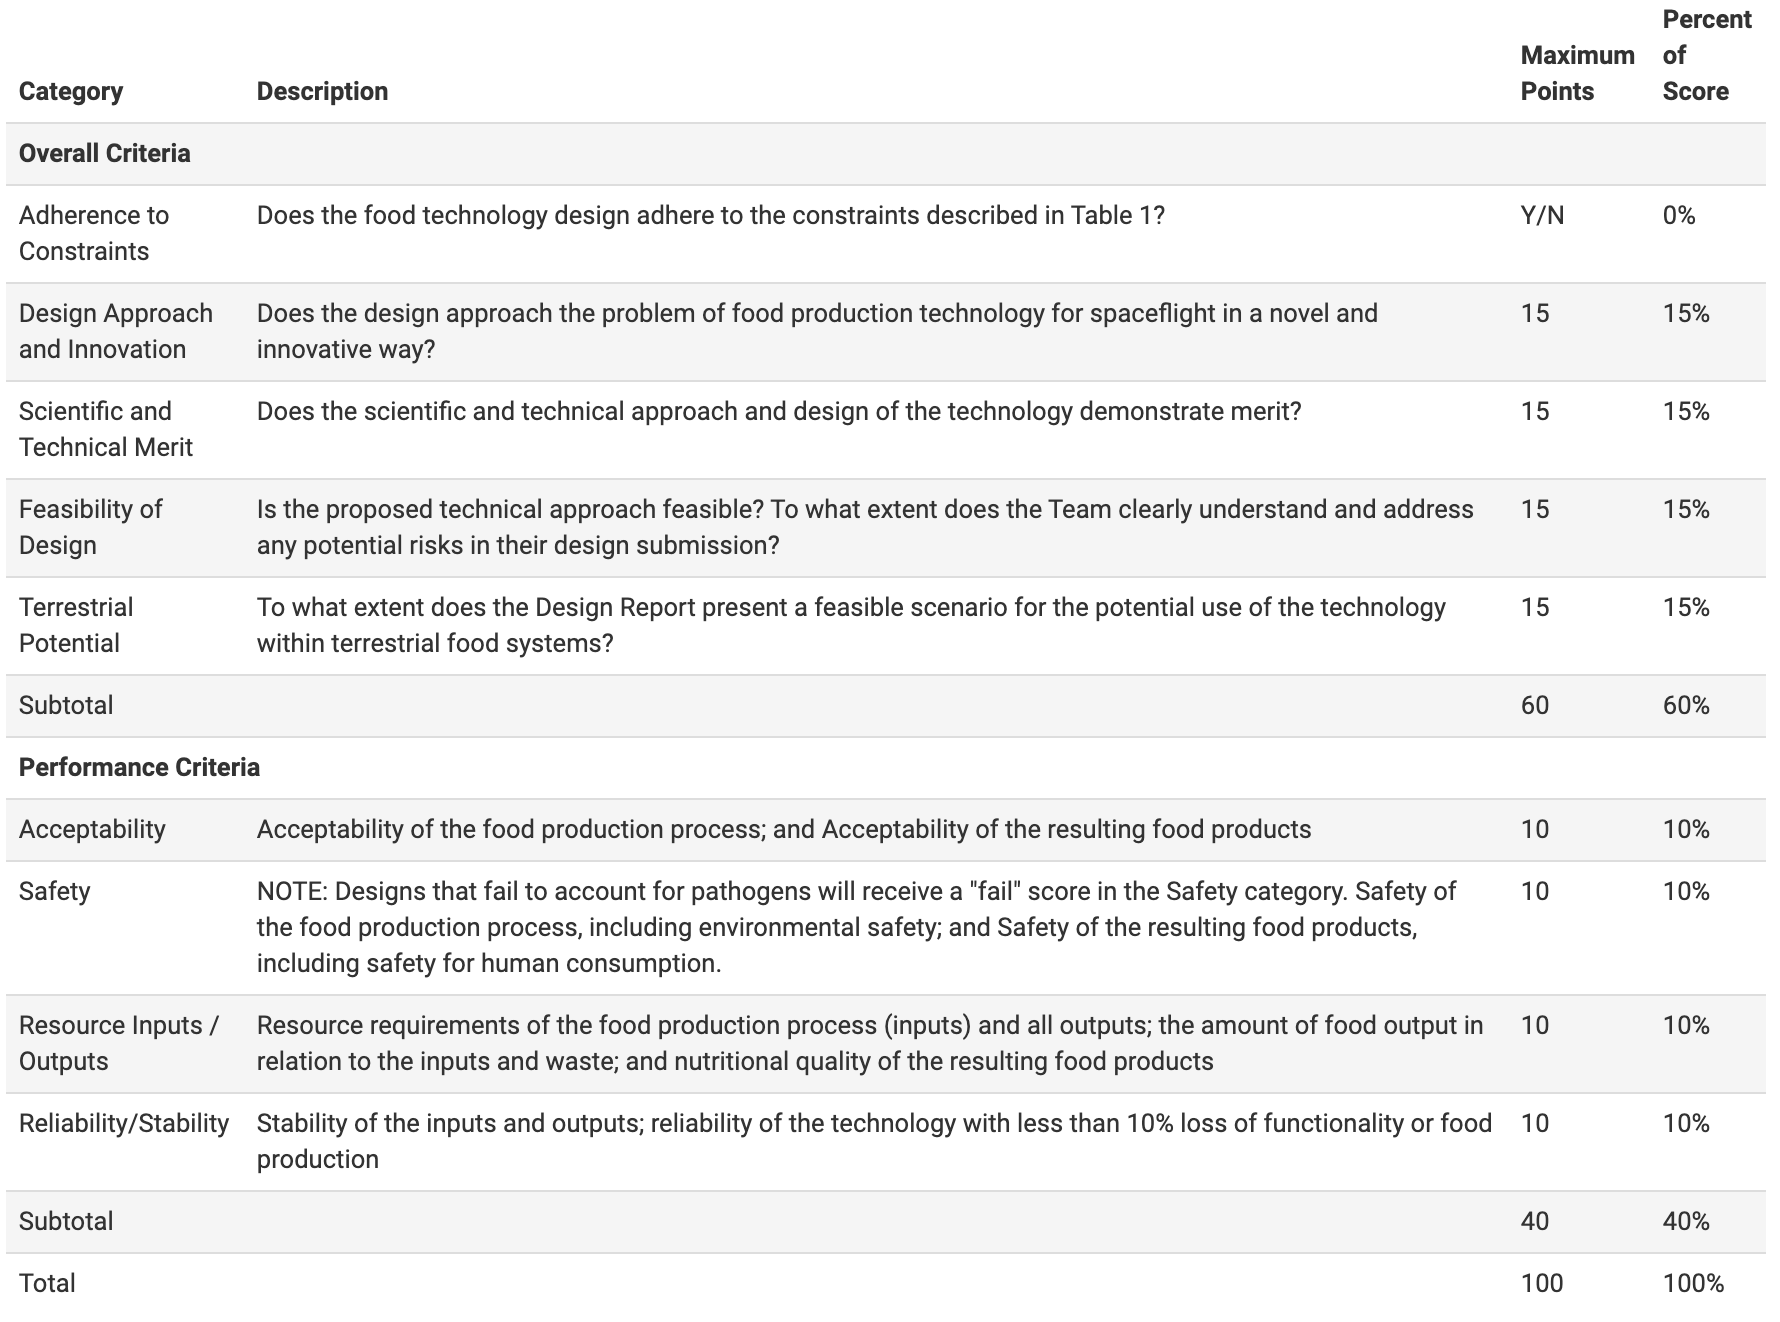
\includegraphics[width=15cm]{images/reportassessment.png}
    \hfill
    \caption{Design report assessment categories and weights \cite{applicantguide}.}
\end{figure}

\subsection{Animation Assessment Criteria}
\label{sec:animassessment}

\begin{figure}[h]
    \centering
    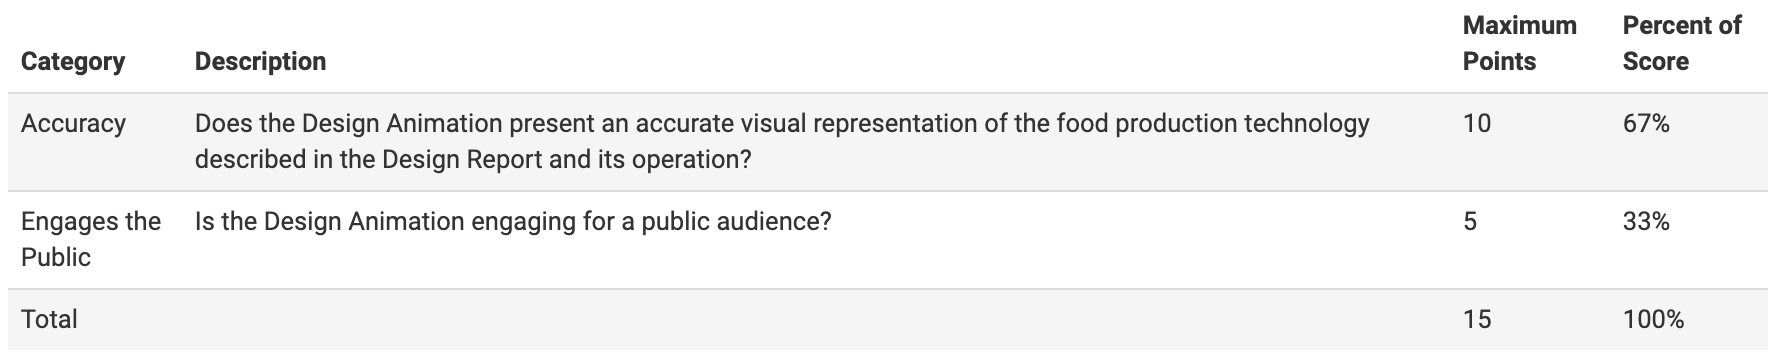
\includegraphics[width=15cm]{images/animassessment.png}
    \hfill
    \caption{Design animation assessment categories and weights \cite{applicantguide}.}
\end{figure}

\newpage
\section{Reference Designs}

% -------- TEMPLATE --------
% Introduction - Project goal, scope, differences from this project
% Graphics - Design drawings/photos, etc.
% Analysis - Rank the design across each of our metrics
    % TODO: Metrics might be too much, maybe just qualitative analysis based on LLOs?

\subsection{Open Agriculture Initiative - Personal Food Computer}

% Project Homepage: https://www.media.mit.edu/groups/open-agriculture-openag/overview/
% Design Repositories: https://github.com/OpenAgricultureFoundation
% PFC White Paper: PDF in Discord
    % Citation: \cite{mit-openag}
% OpenAG White Paper: PDF in Discord
    % Citation: \cite{mit-pfc}

% Half-decent summary: https://www.notion.so/Open-Agriculture-Initiative-OpenAG-cfa5031e2b244093a37158fe1a99ec12

% Introduction

The Open Agriculture Initiative (OpenAG) is a project launched by the MIT Media Lab with the goal to "Build open resources to enable a global community to accelerate digital agricultural innovation." 

One of their primary developments was an open-source controlled-environment agriculture micro-greenhouse, the Personal Food Computer.
The PFC controls all environmental growing parameters and collects data during the growth cycle.
Data can be collected by users and shared between members of the open-source community.
This allows for the creation of reproducible "climate recipes" where other devices with similar abilities can reliably generate the same environment and attain the same plant growth results.

% Graphics

\begin{figure}[h]
    \centering
    \begin{subfigure}[b]{0.08\textwidth}
        \hfill
    \end{subfigure}
    \begin{subfigure}[b]{0.40\textwidth}
        \centering
        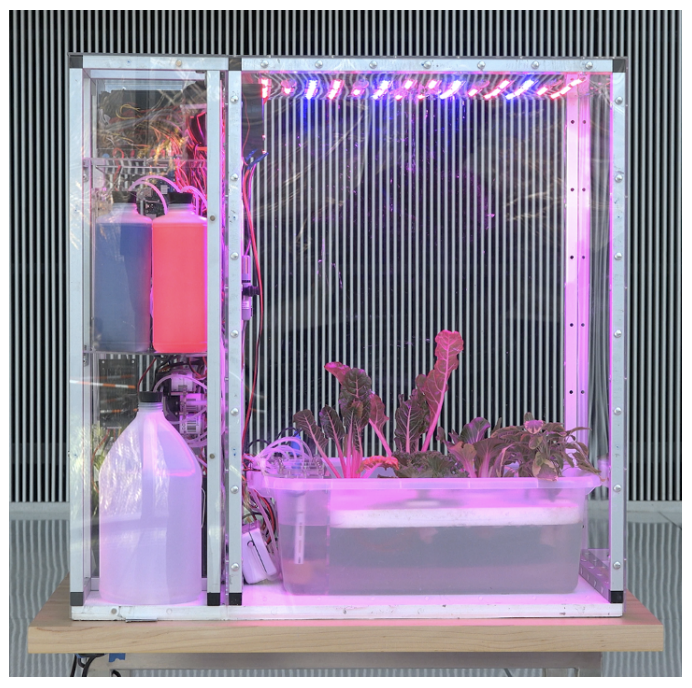
\includegraphics[width=\textwidth]{images/pfc-built.png}
        \caption{Assembled PFC v1.}
        \label{fig:pfc-built}
    \end{subfigure}
    \hfill
    \begin{subfigure}[b]{0.26\textwidth}
        \centering
        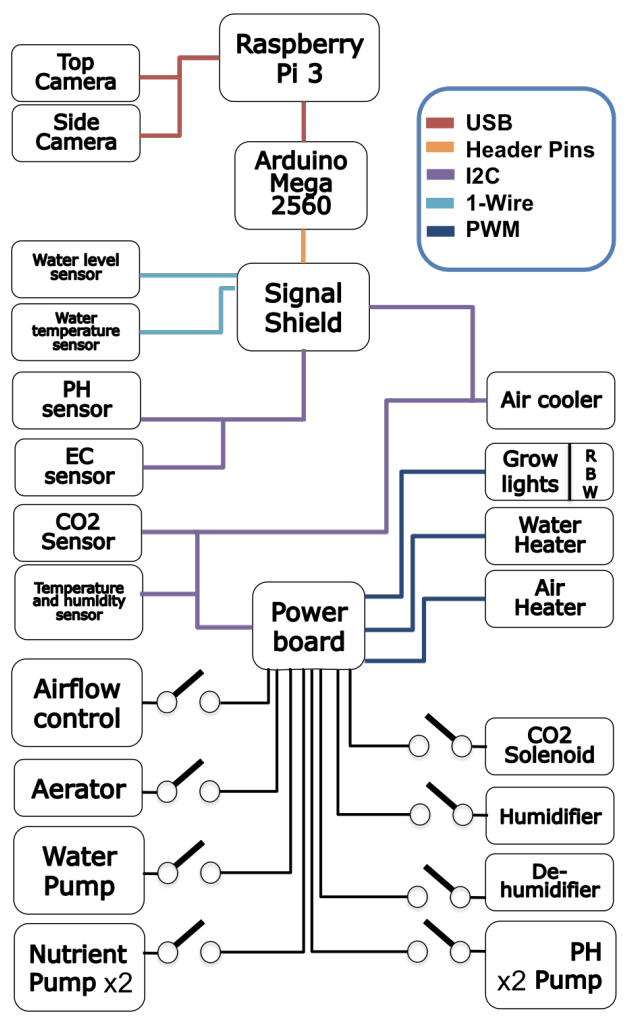
\includegraphics[width=\textwidth]{images/pfc-components.png}
        \caption{Component diagram.}
        \label{fig:pfc-components}
    \end{subfigure}
    \begin{subfigure}[b]{0.10\textwidth}
        \hfill
    \end{subfigure}
    \caption{From \cite{mit-pfc}.}
    \label{fig:pfc}
\end{figure}

One of the design's major flaws is in its implementation. Despite the claim that the PFC focusses on \ref{sc:3} and \ref{sc:5}, in practice, it failed to meet \ref{r:3} \cite{mit-basil}.
In addition, the PFC utilizes Deep Water Culture (DWC) hydroponics \cite{mit-pfc}, as opposed to aeroponics, resulting in a lowered water efficiency.

The PFC is also much more focussed on \ref{sc:3} and \ref{sc:5} than \ref{r:1} and \ref{r:1a}, meaning that they valued optimization and data collection over bulk yield of food outputs. This shows in that their design did not account for scalability of output \cite{mit-wfp}.

However, the array of sensors included in the design (both plant-growth and environmental) as well as the principle of plant phenomenology optimization is informative in meeting \ref{r:3} and their attempts can serve as a basis for understanding \ref{sc:3} and \ref{sc:5} \cite{mit-openag}.

\textbf{Attempted}: \ref{ll:output_variety}, \ref{ll:output_palatability} (via \ref{sc:5}), \ref{ll:control_airtemp}. \ref{ll:control_airhum}, \ref{ll:control_light}, \ref{ll:control_aircirculation}, \ref{ll:control_nutrientsolution}, \ref{ll:automation}

\textbf{Did Not Consider}: \ref{ll:output_energy}, \ref{ll:insulateisolate}, \ref{ll:germinationsuccess}, \ref{ll:efficiency_energy}, \ref{ll:efficiency_water}, \ref{ll:time_germination}, \ref{ll:time_growth}, \ref{ll:time_harvest}, \ref{ll:crosscontamination}

\newpage
\section{Application Details}
\label{sec:application}

The contents of this appendix are adapted from \cite{applicantguide}, and should serve as the framework for developing the Phase 1 prototype.

A complete application package consists of the Challenge Application Form, with the following sections:
\begin{enumerate}
    \item Applicant details (basic information, primary contact);
    \item Proposed solution details:
    \begin{enumerate}
        \item Design Abstract;
        \item Design Report (See Appendix \ref{sec:reportassessment});
        \item Design Animation (See Appendix \ref{sec:animassessment});
        \item Intellectual Property Details;
    \end{enumerate}
    \item Declaration (terms and conditions, Consent for Use, Disclosure and Copyright requirements);
    \item Survey (optional);
\end{enumerate}

\subsection{Design Report Contents}
\label{sec:reportcontents}

\begin{enumerate}
    \item Technology Description
    \begin{enumerate}
        \item Part A (3000 chars) - Form, function, purpose, use;
        \item Part B (1500 chars) - Operations overview with assumptions;
    \end{enumerate}
    \item Innovation - Difference from existing tech w/ examples of novelty, innovation, sustainability;
    \item Adherence to Constraints (300 chars per constraint) - Volume, power, water, mass, data connection, crew time, operational constraints, etc.;
    \item Performance Criteria
    \begin{enumerate}
        \item Acceptability of:
        \begin{enumerate}
            \item Process (3000 chars) - time requirement, procedures, and crew interactions (user-friendliness) in small space (footprint) on a daily basis, incl. setup, maintenance, cleaning, stowage;
            \item Food Products (3000 chars) - appearance, aroma, palatability, flavor, texture;
            \item Additional Comments (1000 chars);
        \end{enumerate}
        \item Safety of:
        \begin{enumerate}
            \item Process (3000 chars) - hazardous compounds used or produced, hazards during cleaning, other process hazards, food handling, and mitigation strategies;
            \item Food Products (3000 chars) - repeated consumption safety as per \cite{nutrition};
            \item Additional Comments (1000 chars);
        \end{enumerate}
        \item Inputs and Outputs
        \begin{enumerate}
            \item Inputs to Technology (3000 chars) - Raw materials, energy, water, etc.;
            \item Outputs and Waste from Technology (3000 chars) - Food products and waste (heat, unusable byproducts, vapours, etc.);
            \item Optimization (1500 chars) - Describe and justify;
            \item Nutrition (3000 chars) - Nutritional potential of tech as per \cite{nutrition};
            \item Additional Comments (1000 chars);
        \end{enumerate}
        \item Reliability and Stability of:
        \begin{enumerate}
            \item Process (3000 chars) - Operational lifespan/functionality loss over time, maintenance (schedule, critical/spare components);
            \item Input and Output (1500 chars) - Input and food output shelf lives and justification;
            \item Additional Comments (1000 chars);
        \end{enumerate}
        \item Terrestrial Potential (3000 chars) - Concrete scenarios/examples of helpful operation.
    \end{enumerate}
\end{enumerate}

\end{appendices}
\newpage

% References
\bibliographystyle{IEEEtran}
\bibliography{references}

\end{document}